\fancyfoot[C]{Kronberger}

%% Human-Computer Interaction System %%%%%%%%%%%%%%%%%%%%%%%

\chapter{Human-Computer Interaction System}

\section{Übersicht}
Das Human-Computer Interaction System ist, wie der Name schon verrät, die Komponente, welche als Schnittstelle zwischen dem Nutzer und dem gesamten elektrischen System dient. Durch es sollte die fehlerfreie Nutzung der Funktionen des Motorrades gewährleistet sein, ebenso sollte es wichtige Fahrdaten und andere Informationen speichern und dem User anzeigen können.\\
Wichtig ist das System, troz der großen Komplexität, so intuitiv und nutzerfreundlich wie möglich zu gestallten.

\subsection{Grundfunktionen des Systems}
Die geplanten Funktionen des HCIS lassen sich grob in vier Grundfunktionen einteilen.
\begin{itemize}
	\item \textbf{Steuerung der Peripherie} \medskip\\
	Die Schalter und Buttons am Lenker, welche zuvor über den Kabelbaum die Leuchten, Blinker oder der Hupe gesteuert haben. Werden nun über die General-purpose input/output (GPIO) anschlüsse des Raspberry Pi Micro Computers gesteuert.
	\item \textbf{Graphische Benutzeroberfäche}\medskip\\
Dient der Anzeige wichtiger Fahr- und Ladedaten welche entweder in echtzeit oder über die Datenbankschnittstelle abgerufen und graphish angezeigt werden können.
	\item \textbf{Kommunikation mit den Steuereinheiten des Motorrades} \medskip\\
	Über CAN-Bus werden Daten von dem Batterie Management Systems (BMS) und der Curtis Motorsteuerung empfangen und an die Benutzeroberfläche zur echtzeit verwertung und an die Datenbankschnittstelle zur Langzeitsicherung der Fahrdaten weiter gegeben.
	\item \textbf{Speichern der relevanten Fahrdaten über die Datenbankschnittstelle} \medskip\\
Die über den CAN-Bus empfangenen Daten werden sofort an die Datenbankschnittstelle (Hander) weitergegeben um für Datenauswertung und Testberichte die Daten zu speichern. Ebenso bezieht das Diagnosesystem der Benutzeroberfläche die Daten über diese Schnittstelle.
\end{itemize}
\newpage

\subsection{Steuereinheit}
Als Basis zur Auswahl der Steuereinheit wurden die zuvor erläuterten Grundfunktionen herangeszogen genommen. Die Ausgewählte Steuereinheit sollte diese erfüllen können und ebenso Potential zur Erweiterung der Funktionen bieten. Genauso wichitg war das eine große Flexibilität und Individualität erreicht werden kann, um nicht in der Umsetzung unserer Ideen eingeschränkt zu sein. Zur Auswahl standen verschiedene Speicherprogrammierbare Steuerungen und Microcomputer, doch letzten endes überzeugte der Micrcomputer Raspberry Pi.

\begin{figure}[H]
	\begin{center}
		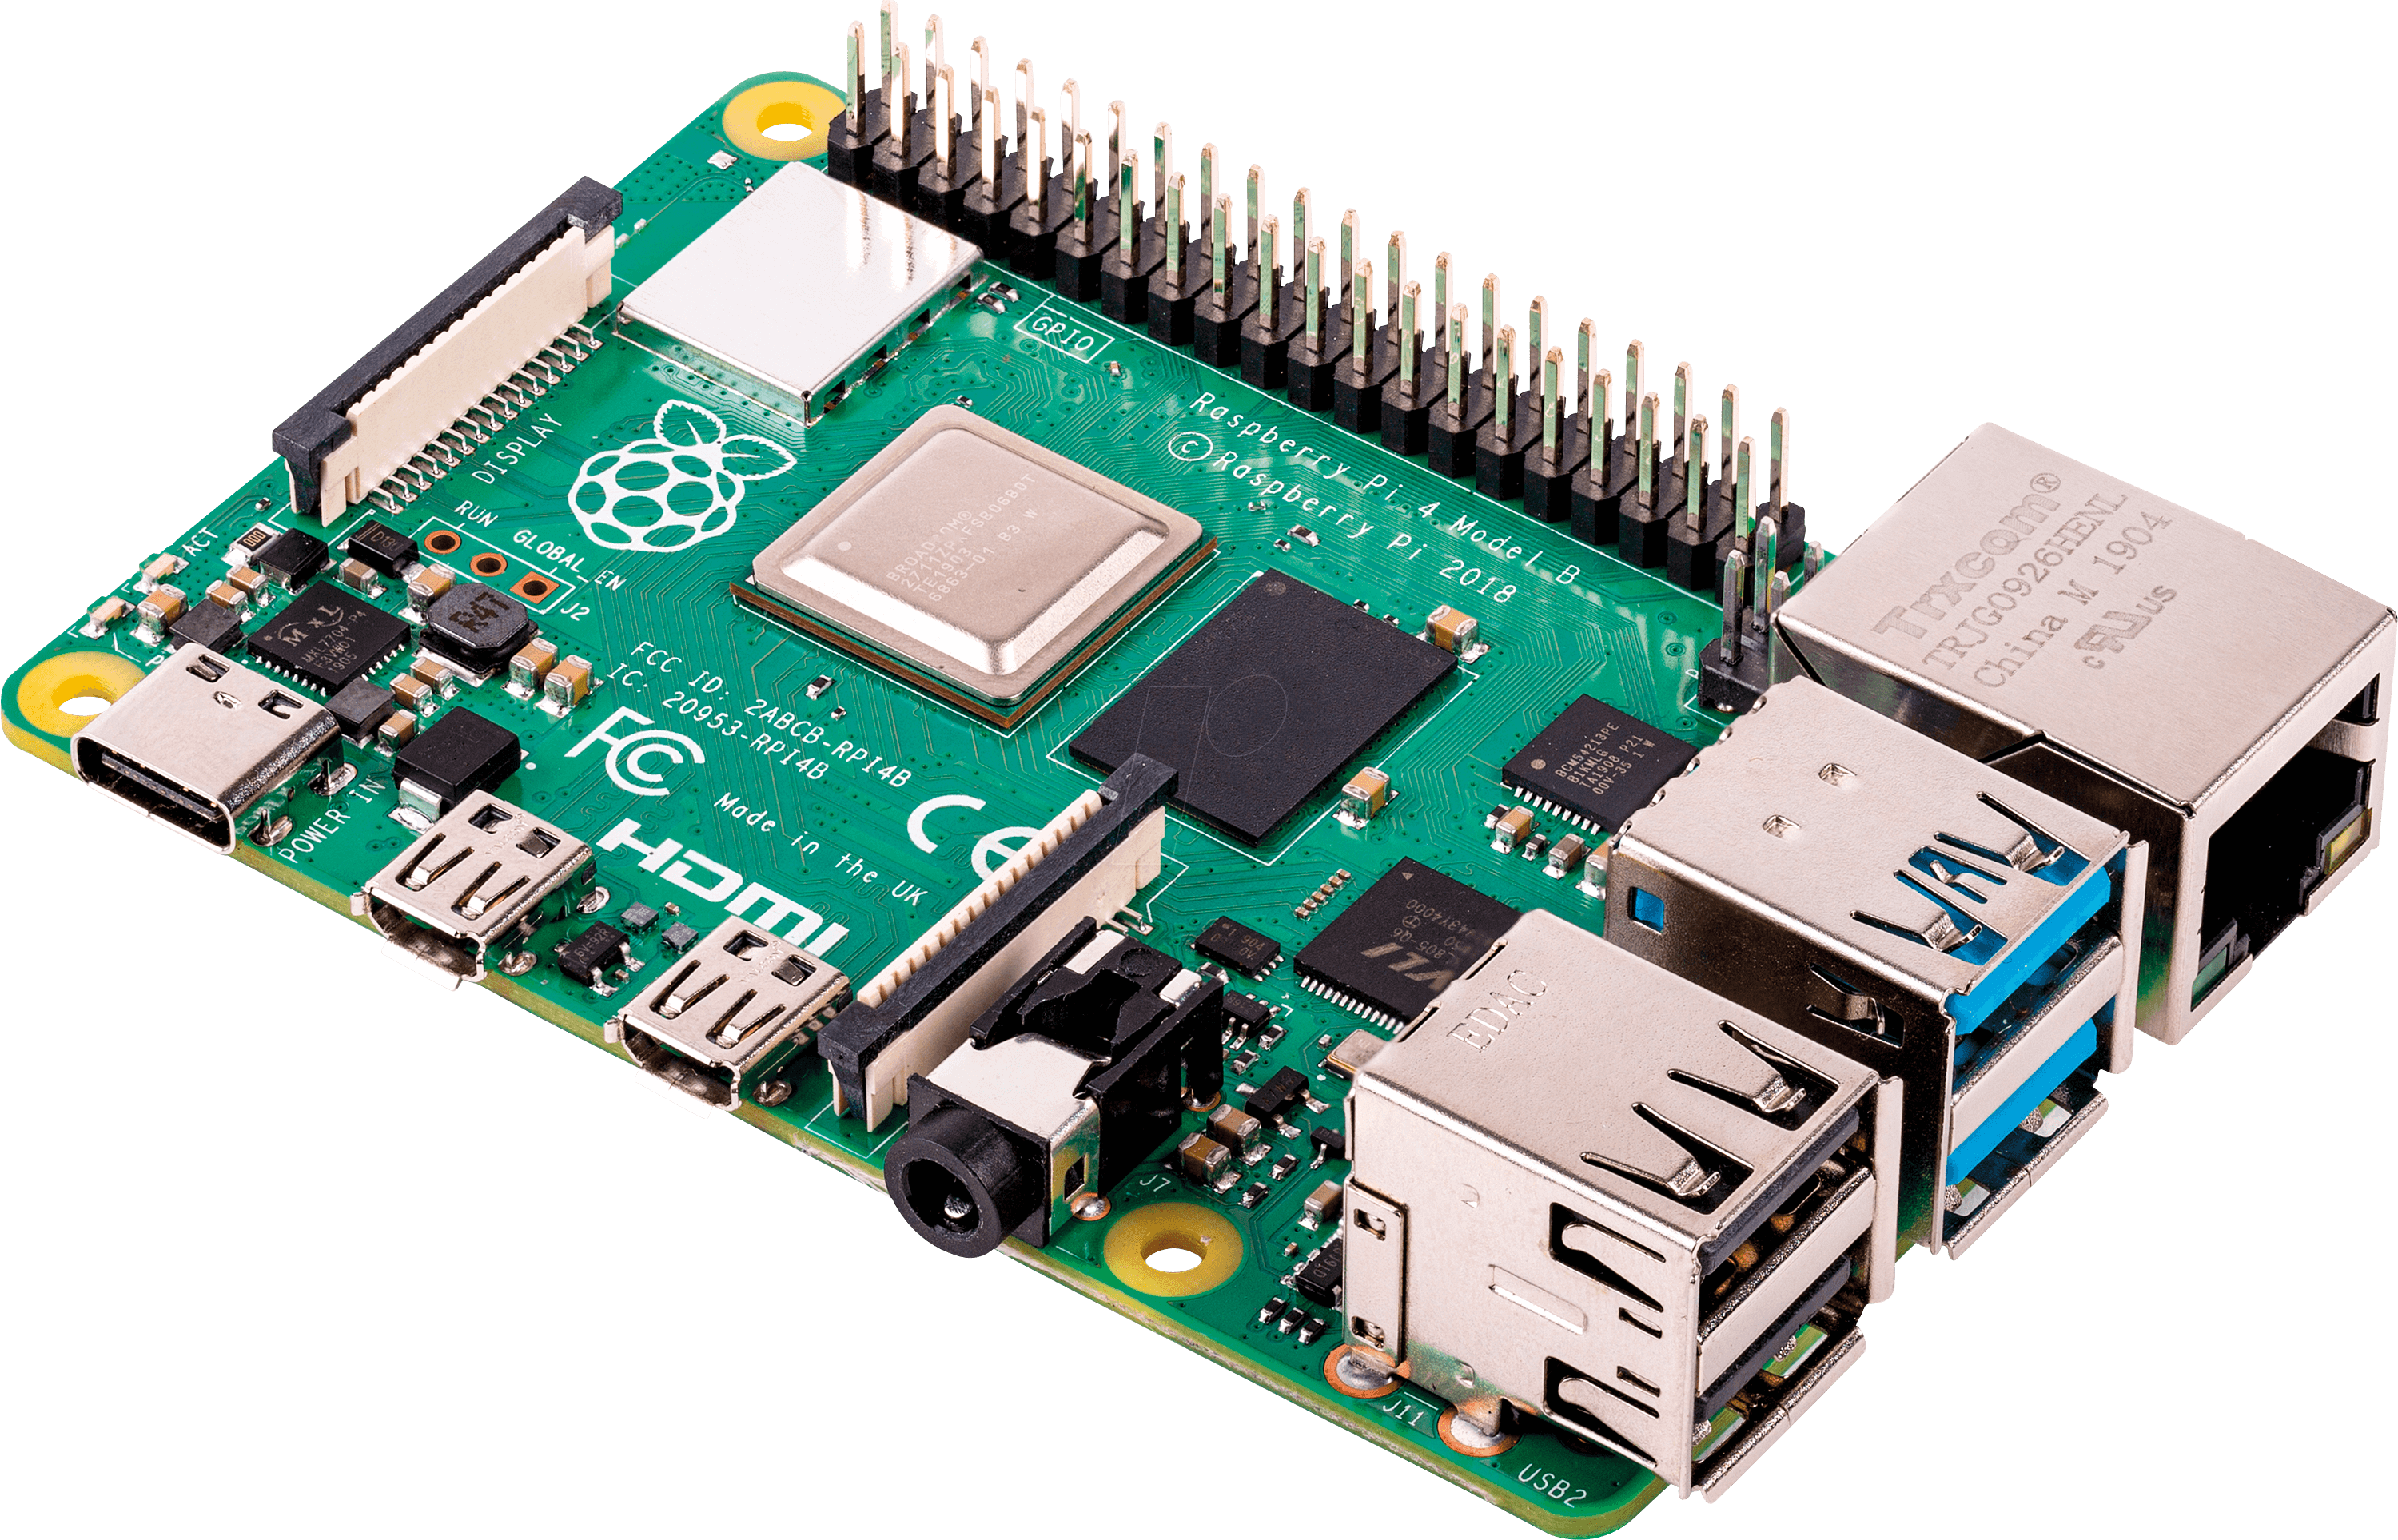
\includegraphics[scale=0.1]{figures/hcis/raspberryPi.png}
		\caption{Raspberry Pi - Steuereinheite des HCIS}
	\end{center}
\end{figure}

Durch 

\newpage

\subsection{Grundaufbau des Systems}
In der Abbildung wird der Grundaufbau des Systems und die Datenverbindungen der folgenden  Komponenten veranschaulicht.

\begin{itemize}
	\item Raspberry Pi - Die Steuereinheit des Systems.
	\\ Kommuniziert über CAN-Bus mit den anderen Steuerkomponenten des Motorrades.
	\item User Input - Die vorhandenen Buttons am Lenker des Motorrads werden über pull down Widerstände mit den Inputs des Raspberry Pi verbunden. 
	\item Peripherie - Die Grundkomponenten des Motorrades wie Scheinwerfer oder Hupe.
	\item Dashboard - Der Bildschirm zur Anzeige der Verarbeiteten Informationen.
\end{itemize}

\begin{figure}[H]
	\begin{center}
		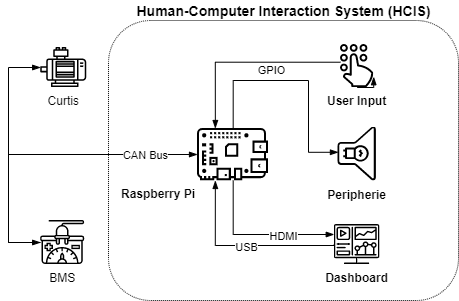
\includegraphics[scale=0.6]{figures/hcis/HCIS_Grundfunktion.png}
		\caption{Grundaufbau des Human-Computer Interaction Systems}
	\end{center}
\end{figure}

Nicht in der Abbildung dargstellt ist die Versorgung der einzelnen Komponenten, welche in dem folgenden Abschnitt noch genauer erläutert wird.

\newpage

%% Versorgung %%%%%%%%%%%%%%%%%%%%%%%%%%%%%%%%%%%%%%%%%%%%%%% 

\section{Versorgung}
\subsection{Aufbau des Versorgungssystems}
\subsection{Spannungswandler}
\subsubsection{5V Versorgungssystem}
\subsubsection{12V Versorgungsysstem}

\newpage

%% Steuerung der Peripherie %%%%%%%%%%%%%%%%%%%%%%%%%%%%%%%%%

\section{Steuerung der Peripherie}
\subsection{Hardware}
\subsubsection{Input}
\subsubsection{Output}

\subsection{Software}
\subsubsection{GPIO Zero}
\subsubsection{Threading}

\newpage

%% Benutzeroberfläche %%%%%%%%%%%%%%%%%%%%%%%%%%%%%%%%%%%%%%%

\section{Benutzeroberfläche}
Die Benutzeroberfläche stellt die Verbindung zwischen dem Nutzer und dem Motorrad dar. Sie sollte während der Fahrt die Instrumententafel des Motorrades zu ersetzen und dem Nutzer die wichtigsten Fahrinformationen anzeigen. Sobald man zum Stillstand gekommen ist, wird es möglich Einstellungen zu ändern und die aufgezeichnetetn Fahrdaten anzeigen zu lassen. Ebenso kann der Akkuladestatus und Informationen über Fehler im System entnommen werden.
\subsection{Hardware}
Zur Anzeige und Bedienung wird ein 11.6 Zoll Kapazitives Touch LCD Display verwendet. Es besitzt eine FullHD Auflösung (1920x1080), was für eine professionelle Darstellung essenttiell ist. Ebenso hat es ein schützendes ABS Gehäuse, welches troz fehlender IPX zertivizierung das Abdichten ermöglicht. Die Versorgungsspannung beträgt 12V, was ident zu den anderen Komponenten am Motorrad ist und daher die Versorgung sehr vereinfacht, kann aslo über den gleichen Spannungswandler versorgt werden.
\subsubsection{Befestigung}

\subsection{Software}
Bevor die Software für die Benutzeroberfläche verfasst wurde, musste das Design, Funktionen sowie die angezeigten Informationen geplant werden, um einen reibungslosen Workflow beim Entwickeln des Front Ends zu gewährleisten. Design Elemente wurden zuvor in Adobe Illustrator vorgefertigt In den Folgenden Seiten wird das Ergebnis dieses Prozesses dargeboten.
\subsubsection{Aufbau}


\subsection{Program Fenster}

\subsubsection{Login}

\begin{figure}[H]
	\begin{center}
		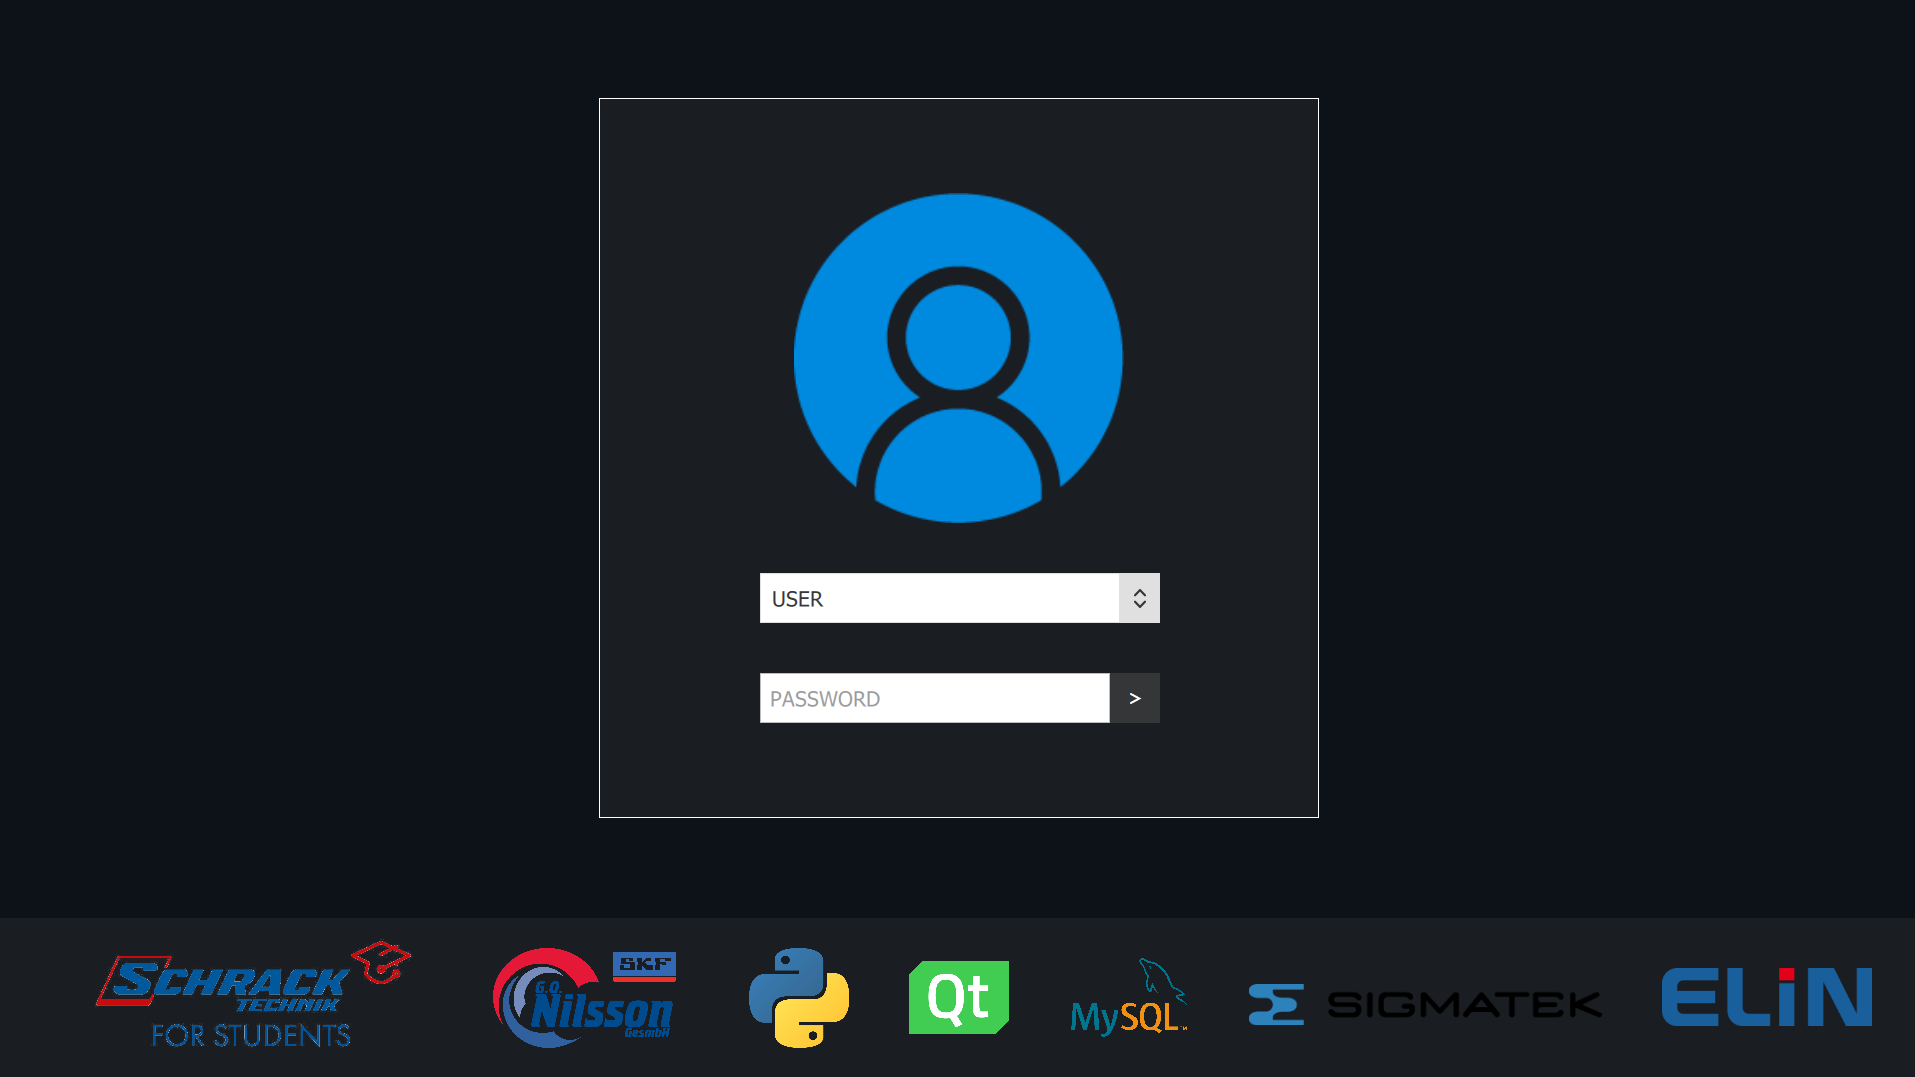
\includegraphics[scale=0.24]{figures/hcis/window_login.png}
		\caption{GUI Fenster - Login Menu}
	\end{center}
\end{figure}

\subsubsection{Fahrdaten}

\begin{figure}[H]
	\begin{center}
		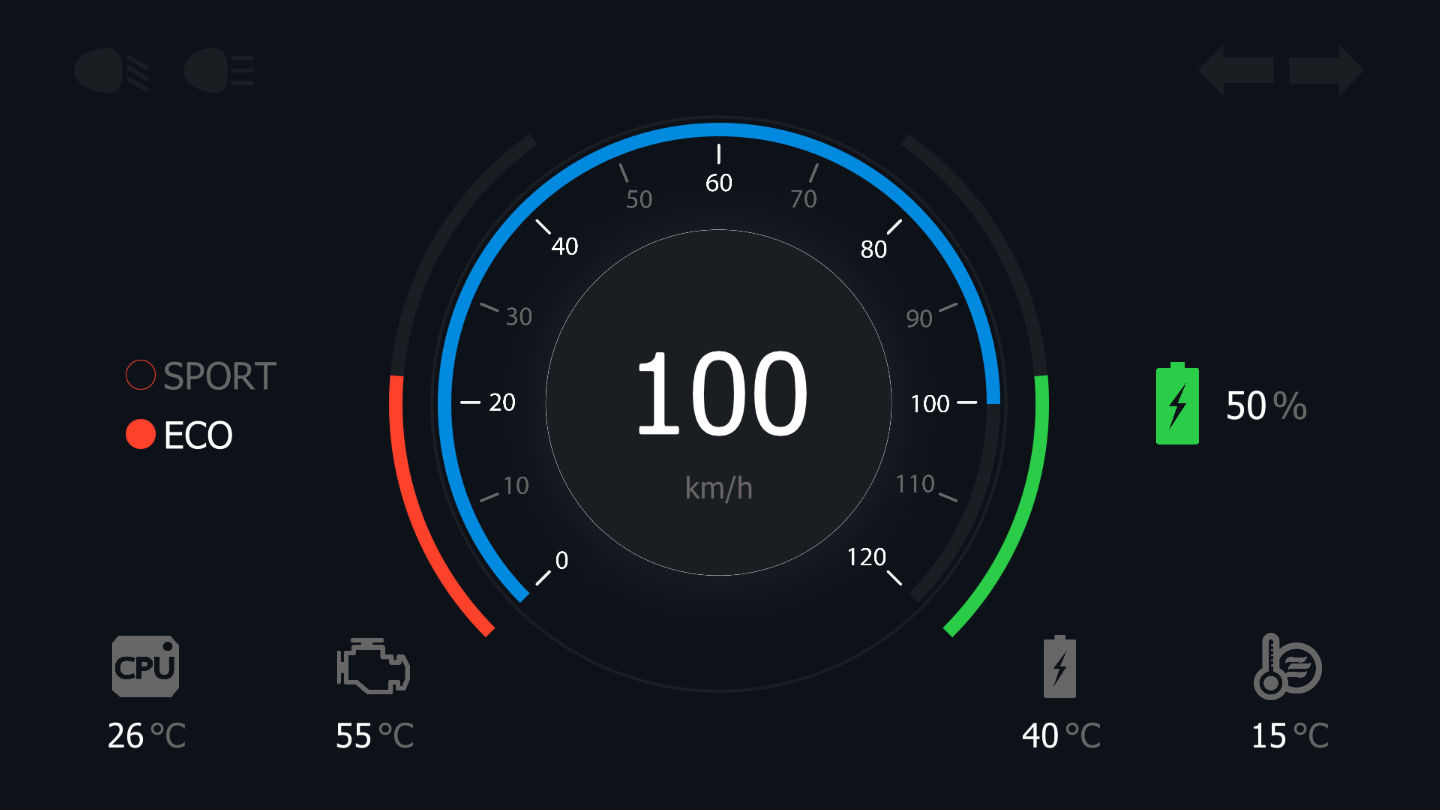
\includegraphics[scale=0.24]{figures/hcis/window_dashboard.png}
		\caption{GUI Fenster - Fahrdaten}
	\end{center}
\end{figure}

\newpage

\subsubsection{Akku- und Ladedaten}

\begin{figure}[H]
	\begin{center}
		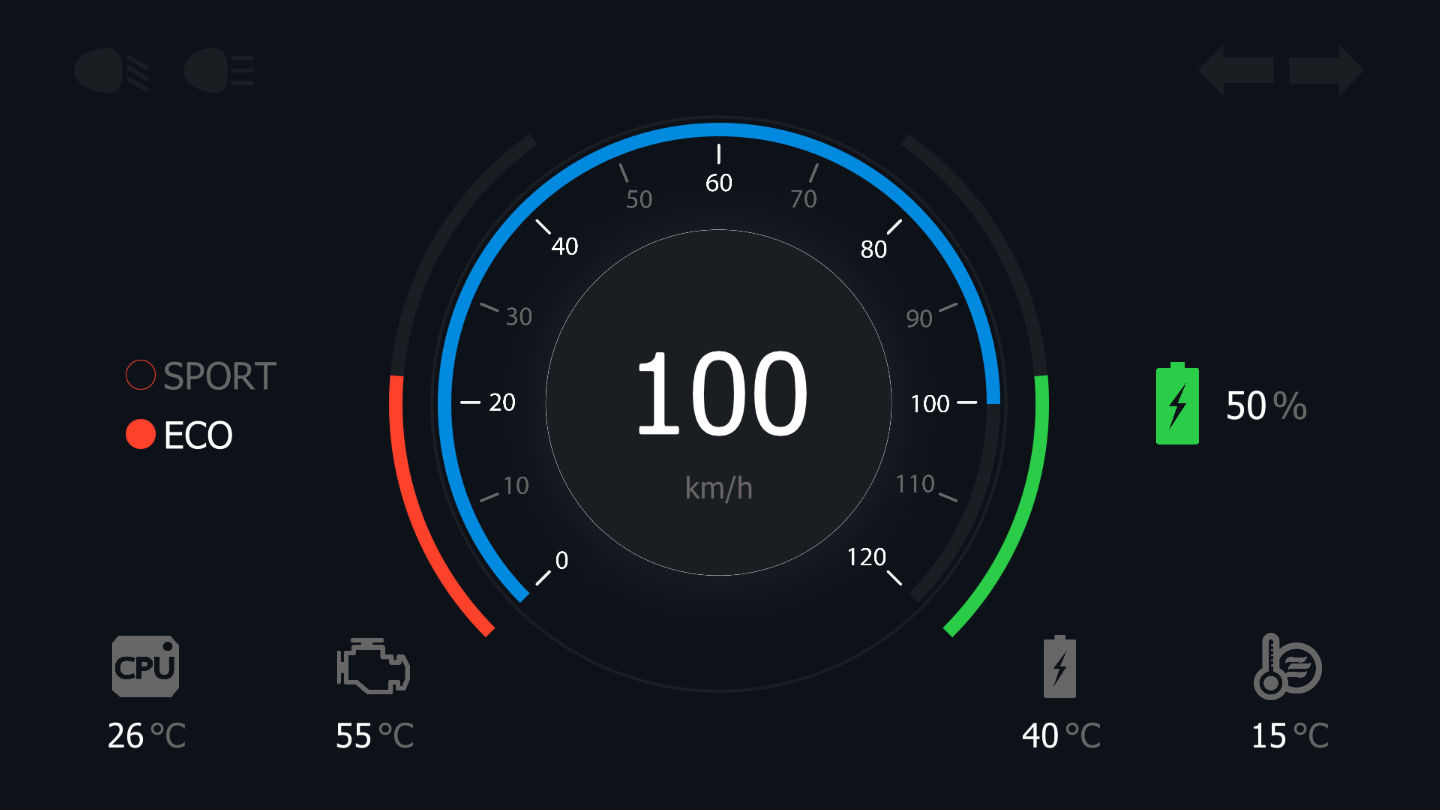
\includegraphics[scale=0.24]{figures/hcis/window_dashboard.png}
		\caption{GUI Fenster - Akkudaten}
	\end{center}
\end{figure}

\subsubsection{Fahrdaten Diagnose}

\begin{figure}[H]
	\begin{center}
		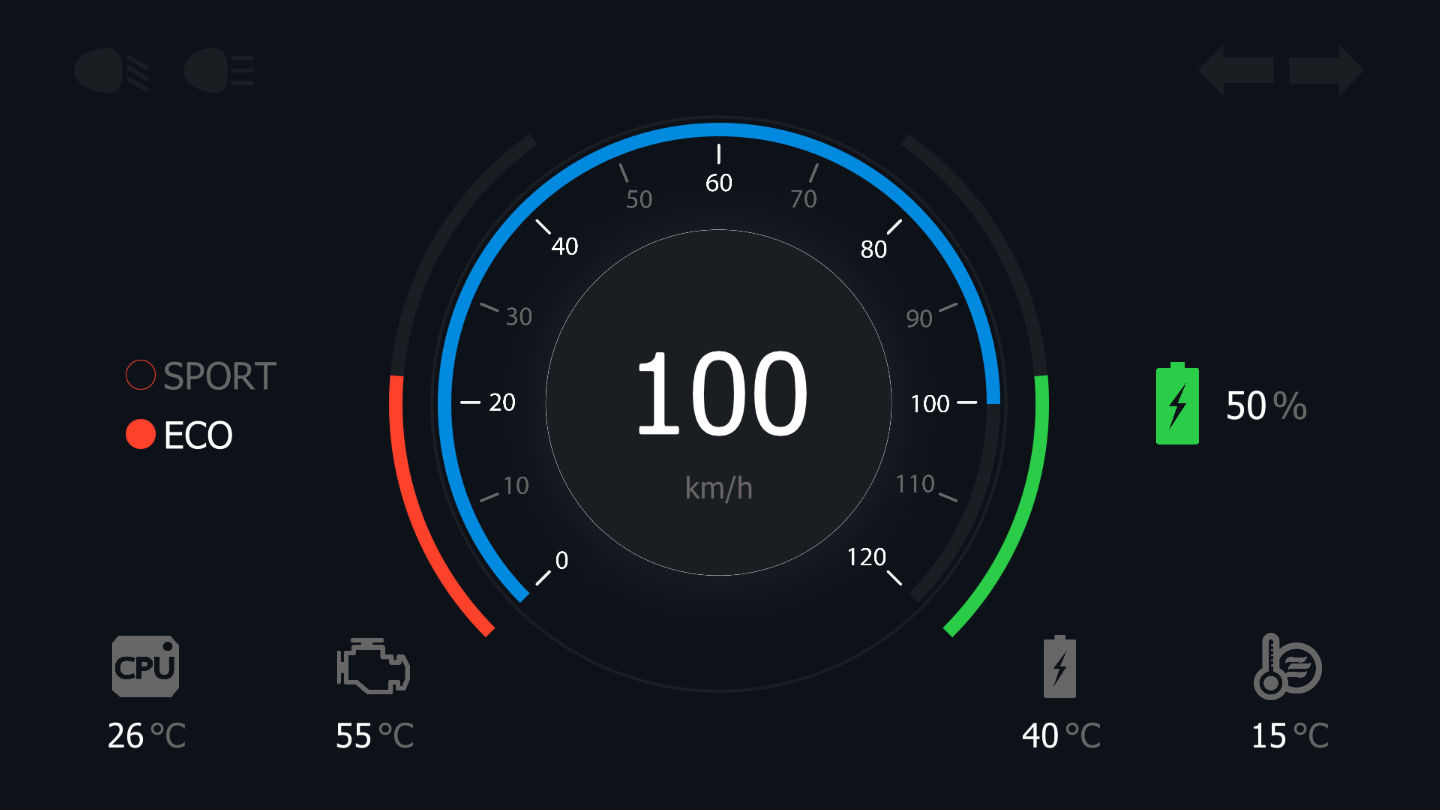
\includegraphics[scale=0.24]{figures/hcis/window_dashboard.png}
		\caption{GUI Fenster - Fahrdaten Diagnose}
	\end{center}
\end{figure}

\subsubsection{Errors}

\begin{figure}[H]
	\begin{center}
		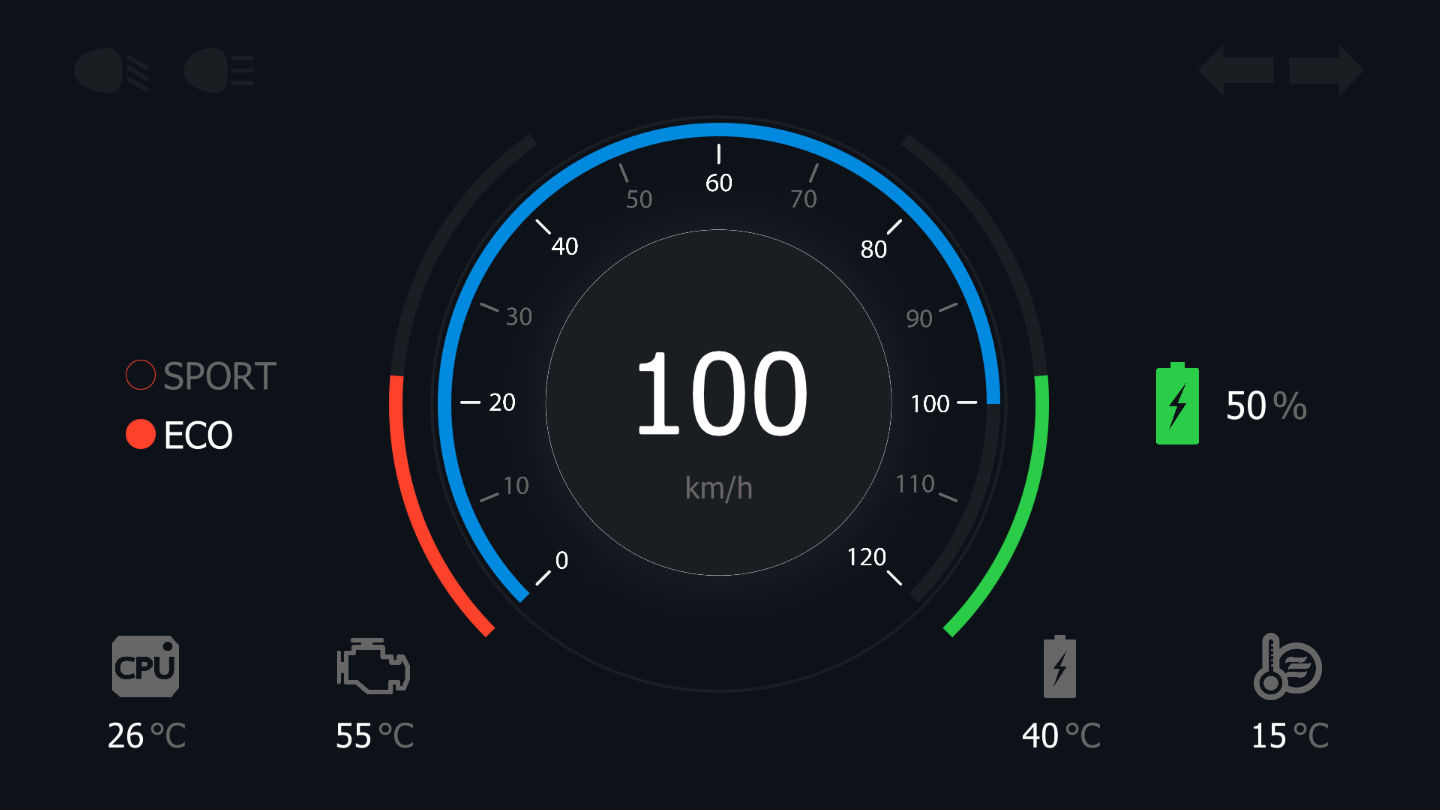
\includegraphics[scale=0.24]{figures/hcis/window_dashboard.png}
		\caption{GUI Fenster - Error List}
	\end{center}
\end{figure}

\subsection{Komponenten}

\subsubsection{Navigations Menu}

\begin{figure}[H]
	\begin{center}
		
\includegraphics[scale=0.2]{figures/hcis/component_menu.png}
		\caption{GUI Komponente - Navigation Menu}
	\end{center}
\end{figure}

\subsubsection{Balken Anzeige}

\begin{figure}[H]
	\begin{center}
		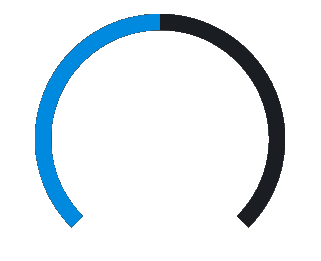
\includegraphics[scale=0.4]{figures/hcis/component_bar.png}
		\caption{GUI Komponente - Balken Anzeige}
	\end{center}
\end{figure}

\newpage

\subsection{Realisierung der Benutzeroberfäche}

\subsubsection{QML}
QML ist eine deklarative Sprache, mit der Benutzeroberflächen anhand ihrer visuellen Komponenten und ihrer Interaktion und Beziehung zueinander beschrieben werden können. Es ist eine gut lesbare Sprache, die entwickelt wurde, um die dynamische Verbindung von Komponenten zu ermöglichen, und die die einfache Wiederverwendung und Anpassung von Komponenten innerhalb einer Benutzeroberfläche ermöglicht. Es bietet eine gut lesbare, deklarative, Syntax mit Unterstützung für JavaScript-Ausdrücke in Kombination mit dynamischen Eigenschaftsverbindungen.

\subsubsection{Qt-Quick}
Das Qt-Quick-Modul ist die Standardbibliothek zum schreiben von QML-Anwendungen. Während das QML-Modul die Engine und die Sprachinfrastruktur bereitstellt, bietet das Qt Quick-Modul alle grundlegenden Typen, die zum Erstellen von Benutzeroberflächen mit QML erforderlich sind. Es bietet eine visuelle Zeichenfläche und Typen zum Erstellen und Animieren visueller Komponenten, zum Empfangen von Benutzereingaben, zum Erstellen von Datenmodellen und Ansichten sowie zum verzögerten Objektinstanziieren. Es können problemlos flüssige, animierte Benutzeroberflächen in QML erstellt werden. Diese Benutzeroberflächen können mit beliebigen Back-End Bibliotheken verbunden werden.

\subsubsection{Slots und Signals}
Slots und Signals werden in Qml zur ereignisgesteuerte Kommunikation zwischen front-end und back-end verwendet. In der folgenden Illustration wird diese anhang eines einfachen Beispiels erklärt.

\begin{figure}[H]
\begin{center}
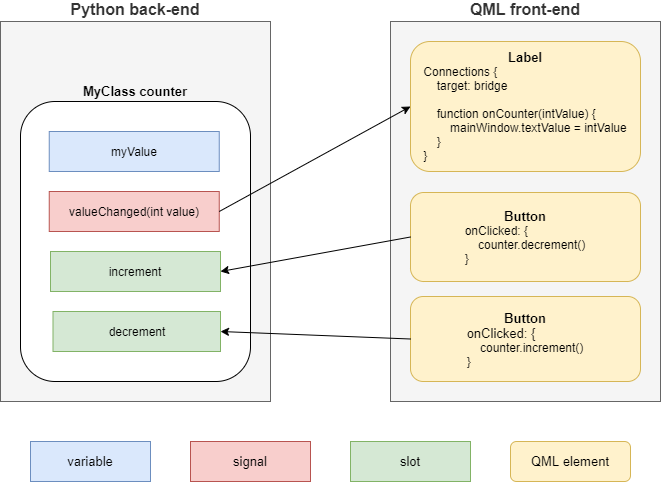
\includegraphics[scale=0.4]{figures/hcis/signals_slots.png}
\caption{Slots und Signals Konzept}
\end{center}
\end{figure}

\textbf{Signale}\\ \medskip
Diese können als Mitteilungen angesehen werden welche über das Aufrufen der signal.emit funktion vom back-end an das front-end gesehendet wird. Im front-end wird wiederum eine eigens definierte Funktion benötigt um dem Wert einem Property eines QML Elements zuzuweisen.
\medskip

\textbf{Slots}\\ \medskip
Slots sind Call-Back Funktionen, welche im Back-End definiert werden und sind über die Bridge Class mit dem Front-End verknüpft. Dadurch können diese Funktionen im Front-End aufgerufen und mit Signalen verbunden werden. Sie stellen daher die wichtigste Verbindung zwischen dem Programm und der Benutzeroberfläche dar.

\newpage
	
\subsubsection{Bridge}

\newpage

%% Kommunikation %%%%%%%%%%%%%%%%%%%%%%%%%%%%%%%%%%%%%%%%%%%%

\section{Kommunikation}
Um Daten zwischen den mehreren Steuereinheiten des Motorrades zu versenden muss eine echtzeit Kommunikation über ein Bussystem gewährleistet werden. Die Entscheindung ist auf das Controller Area Network Bussystem (CAN-Bus) gefallen. Auschlaggebend für diese Entscheidung war der Curtis Motorcontroller, denn dieser verfügt über eine serielle Schnittstelle (RS-232) sowie ein CAN-System. Für unserer Anwendung bietet das CAN-System eine größere Ausbaufähigkeit sowie größere Übertragungsraten, weshalb wir uns letztendlich auch dafür entschieden haben.
\subsection{Hardware}
\subsubsection{CAN-Modul}
Da der Raspberry Pi selbst nicht über ein CAN-System verfügt, erfolgt der Anschluss an die Busleitung über ein externes CAN-Modul, welches über das Serial Peripheral Interface (SPI) mit dem Raspberry kommuniziert, welches wie folgt angeschlossen werden muss: 
\begin{figure}[H]
	\begin{center}
		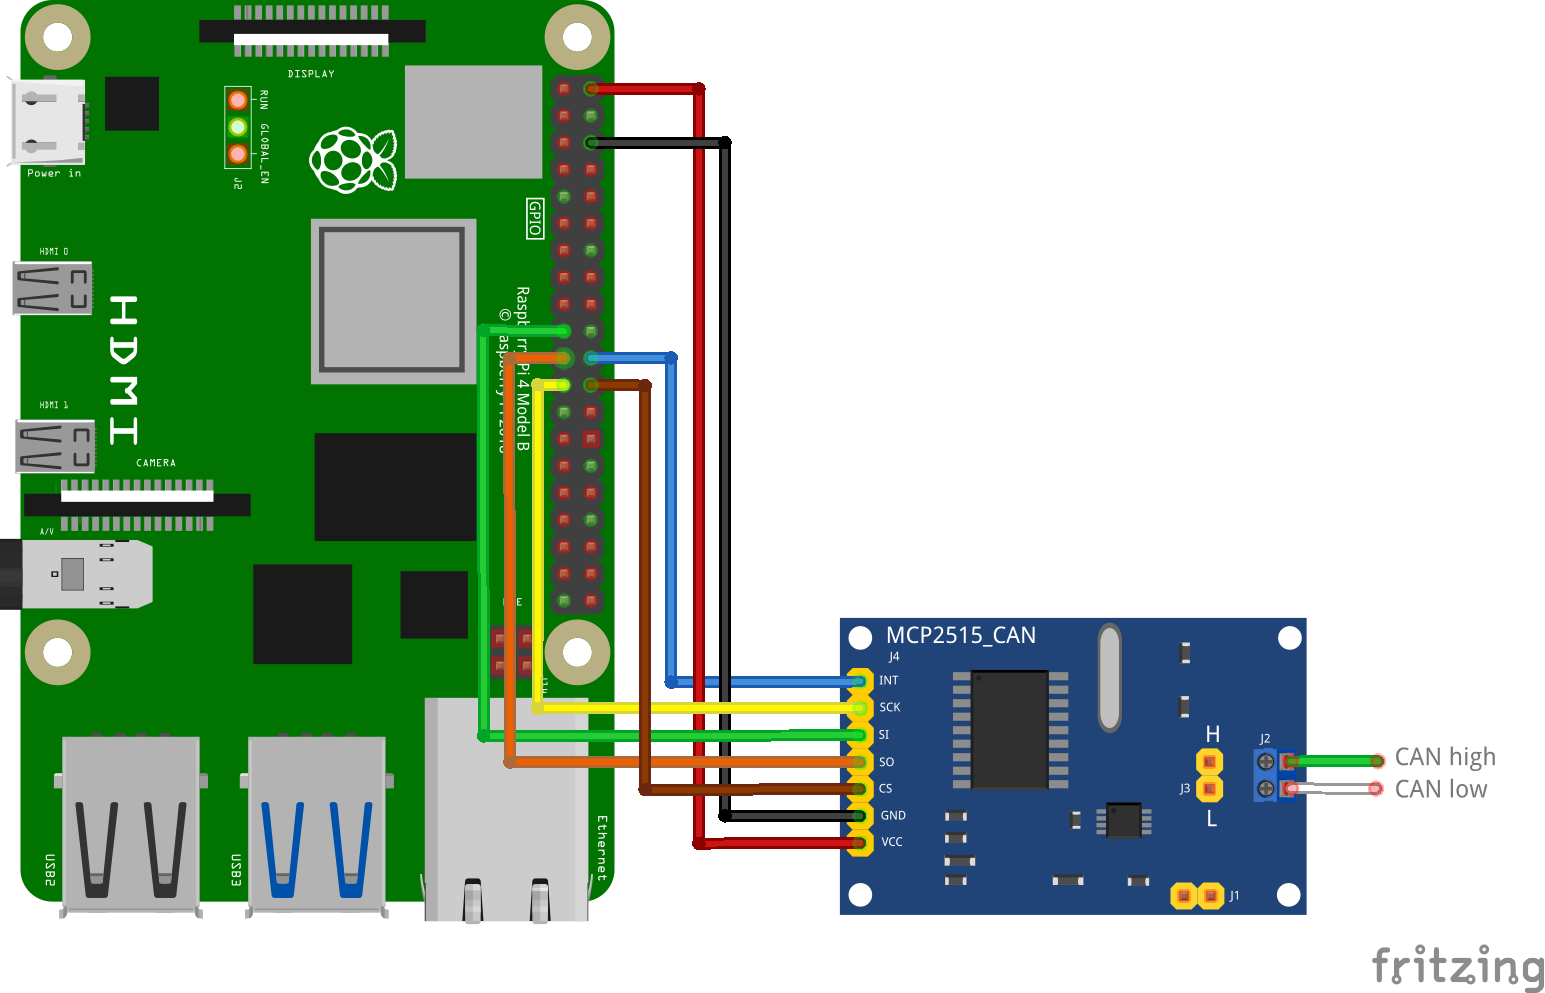
\includegraphics[scale=0.9]{figures/hcis/can_module.png}
		\caption{Anschlussplan CAN-Modul}
	\end{center}
\end{figure}

Die Kommunikation wird über zwei Komponenten ermöclicht. Einen MCP2562 Transceiver, welcher für die Verabeitung der Nachrichten zuständig ist und ein MCP2515 CAN Interface, welches die Daten zwischenspeichert und sich um das Versenden der Nachrichten kümmert. Gemeinsam mit dem Mircocomputer ergibt dies nun eine CAN Node, welche fähig ist Nachrichten zu versenden und zu Empfangen.
\subsubsection{Netzwerkstruktur}
Ein CAN-Netzwerk wird standartmäßig als Linienstuktur oder Sternsturktur aufgebaut. Wir haben uns bewusst für ein Liniensystem entschieden da Sternsysteme nur in bestimmten anwendungen gebrauch finden und noch dazu markante Nachteile besitzt.\\ Es müsste zum Beispiel eine Zentrale Steuereinheit den Nachrichten verkehr steuern, ebenso gibt uns die niedrige Anzahl an Teilnehmern im Netzwerk nicht einmal die Freiheit dazu ein anderes system anzustreben. Erst falls wir in Zukunft das CAN-Netwerk um Sensoren und Aktoren erweitern wollten, müsste weitere Zeit in die Planung des Netzwerks gesteckt werden. 

\newpage

\subsection{Listener}
\subsubsection{Receive Data}


%% Fahrdatenspeicher %%%%%%%%%%%%%%%%%%%%%%%%%%%%%%%%%%%%%%%%

\section{Fahrdatenspeicher}
\subsection{Datenbankstruktur}
\subsubsection{Login System}
\subsubsection{Motor Daten}
\subsubsection{Akku Daten}
\subsection{Handler}
\subsubsection{SELECT Befehl}
\subsubsection{INSERT Befehl}

\newpage